\begin{figure}[ht]
\begin{center}
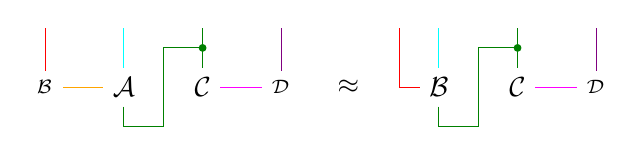
\begin{tikzpicture}[x=1cm,y=1cm]
  \node (sb1) at (0,1) {$\simul_{\mathcal{B}}$};
  \node (a1) at (1,1) {$\mathcal{A}$};
  \node (c1) at (2,1) {$\mathcal{C}$};
  \node (sd1) at (3,1) {$\simul_{\mathcal{D}}$};
  \draw[color=Red] (0,1.75) -- (sb1.north);
  \draw[color=Cyan] (1,1.75) -- (a1.north);
  \draw[color=Green] (2,1.75) -- (c1.north);
  \draw[color=Green] (a1.south) -- (1,.5) -- (1.5,.5) -- (1.5,1.5) -- (2,1.5);
  \draw[color=Magenta] (c1.east) -- (sd1.west);
  \draw[color=Purple] (sd1.north) -- (3,1.75);
  \draw[color=Orange] (sb1.east) -- (a1.west);
  \node[circle,fill,inner sep=1pt,color=Green] at (2,1.5) {};

  \node (b2) at (5,1) {$\mathcal{B}$};
  \node (c2) at (6,1) {$\mathcal{C}$};
  \node (sd2) at (7,1) {$\simul_{\mathcal{D}}$};
  \draw[color=Red] (4.5,1.75) -- (4.5,1) -- (b2.west);
  \draw[color=Cyan] (5,1.75) -- (b2.north);
  \draw[color=Green] (6,1.75) -- (c2.north);
  \draw[color=Green] (b2.south) -- (5,.5) -- (5.5,.5) -- (5.5,1.5) -- (6,1.5);
  \draw[color=Magenta] (c2.east) -- (sd2.west);
  \draw[color=Purple] (sd2.north) -- (7,1.75);
  \node[circle,fill,inner sep=1pt,color=Green] at (6,1.5) {};
  \node at (3.85,1) {$\approx$};
\end{tikzpicture}
\end{center}
\caption{Visual equivalence for substituting the main protocol $\mathcal{B}$.}
\label{fig:commucstep2}
\end{figure}

%%% Local Variables:
%%% mode: latex
%%% TeX-master: "../main"
%%% End:
